\documentclass[a4paper,11pt,twocolumn]{article}

\usepackage{amsmath}
\usepackage[english]{babel}
\usepackage[style=ieee,backend=bibtex]{biblatex}
	\bibliography{references.bib}
\usepackage{booktabs}
\usepackage[font={small},labelfont=sc]{caption}
\usepackage{helvet}
\usepackage[hidelinks]{hyperref}
\usepackage{geometry}
\usepackage{fancyhdr}
\usepackage{float}
\usepackage{graphicx}
\usepackage[latin1]{inputenc}
\usepackage{nomencl}
	\setlength{\nomitemsep}{0pt}
	\makenomenclature
\usepackage{microtype}
\usepackage{pgfplots}
    \pgfplotsset{compat=1.15}
\usepackage{siunitx}
\usepackage{threeparttable}
\usepackage{tikz}
	\usetikzlibrary{calc}
    \usetikzlibrary{external}
    	\tikzexternalize[prefix=tikz/]
	\usetikzlibrary{positioning}
	\usetikzlibrary{shapes.misc}
\usepackage{titling}
\usepackage{xspace}

\renewcommand{\sfdefault}{phv}
\renewcommand{\familydefault}{\sfdefault}

\newcommand{\Matlab}{\textsc{Matlab}\textsuperscript{\textregistered}\xspace}
\newcommand{\sse}{\textsc{sse}\xspace}
\newcommand{\Sse}{\textsc{Sse}\xspace}

\title{Controller Design in \Matlab}
\author{Z0996690}
\date{\today}

\pagestyle{fancy}
\fancyhf{}
\lhead{\includegraphics[width=0.1\textwidth]{img/Durham.png}}
\chead{\thetitle}
\rhead{\theauthor}
\cfoot{\thepage}

\begin{document}

% Title page.
\begin{titlepage}
    \centering
    \vspace*{\fill}
    \includegraphics[width=0.5\textwidth]{img/Durham.png}\\
    \vspace*{\fill}
    \LARGE\thetitle\\
    \vskip0.2em
    \large Level 3 Control and Signal Processing\\
    \vskip0.4em
    \large\theauthor\\
    \vskip0.4em
    \large\thedate\\
    \vspace*{\fill}
\end{titlepage}

% Abstract
\twocolumn[{%
\begin{@twocolumnfalse} \centering
    \renewcommand{\abstractname}{\large Abstract}
    \begin{abstract}
        This report describes the design of two controllers for an industrial plant process in \Matlab. Each controller was designed to meet a different performance specification.
    \end{abstract}
    \vskip\parsep
\end{@twocolumnfalse}
}]

% Acronyms
% Lowercase latin
\nomenclature[1s]{$s$}{Laplace domain variable\hfill[\si{\radian\per\second}]}
\nomenclature[1t]{$t$}{Time domain variable\hfill[\si{\second}]}

% Lowercase greek
\nomenclature[2f]{$\zeta$}{Damping factor}
\nomenclature[2f]{$\omega_n$}{Natural frequency}

% Uppercase latin
\nomenclature[4G]{$G$}{Industrial plant process transfer function}
\nomenclature[4Gc]{$G_c$}{Controller transfer function}
\nomenclature[4L]{$\mathcal{L}$}{Laplace transform operator}
\nomenclature[4M0]{$M_0$}{Peak overshoot}
\nomenclature[4SSE]{$SSE$}{Steady state error}
\nomenclature[4Tr]{$T_r$}{Rise time\hfill[\si{\second}]}
\nomenclature[4Ts]{$T_s$}{Two percent settling time\hfill[\si{\second}]}

% Uppercase greek
\printnomenclature

\section{Introduction}
\section{Background}

Figure~\ref{fig:closed} illustrates a closed loop system. The controller is designed to drive the output $y(s)$ of the plant process to the desired output $r(s)$.

\begin{figure}[h]
	\centering
	\footnotesize
	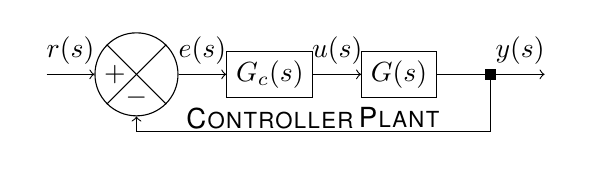
\begin{tikzpicture}[node distance=0.05\textwidth and 0.05\textwidth]
		\node (desire) {};
		\node [draw,right=of desire,circle,minimum size=3em] (sum) {};
			\draw (sum.north west) -- (sum.south east);
			\draw (sum.north east) -- (sum.south west);
		\node [draw,right=of sum,rectangle] (controller) {$G_c(s)$};
		\node [draw,right=of controller,rectangle] (plant) {$G(s)$};
		\node [fill,right=of plant,rectangle,inner sep=2pt] (branch) {};
		\node [right=of branch] (output) {};
		\node [below=of branch.center] (feedback1) {};
		\node [below=of sum.center] (feedback2) {};

		\draw [->] (desire) -- (sum);
		\draw [->] (sum) -- (controller);
		\draw [->] (controller) -- (plant);
		\draw [->] (plant) -- (output);
		\draw [->] (branch) -- (feedback1.center) -- (feedback2.center) -- (sum);

		\node [anchor=west] at (sum.west) {$+$};
		\node [anchor=south] at (sum.south) {$-$};

		\node [anchor=south west] at (desire) {$r(s)$};
		\node [anchor=south] at ($(sum.east)!0.5!(controller.west)$) {$e(s)$};
		\node [anchor=south] at ($(controller.east)!0.5!(plant.west)$) {$u(s)$};
		\node [anchor=south east] at (output) {$y(s)$};

		\node [anchor=north] at (controller.south) {\textsc{Controller}};
		\node [anchor=north] at (plant.south) {\textsc{Plant}};
	\end{tikzpicture}
	\caption{Block diagram of the closed loop system.}
	\label{fig:closed}
\end{figure}

\begin{figure}[h]
	\centering
	\footnotesize
	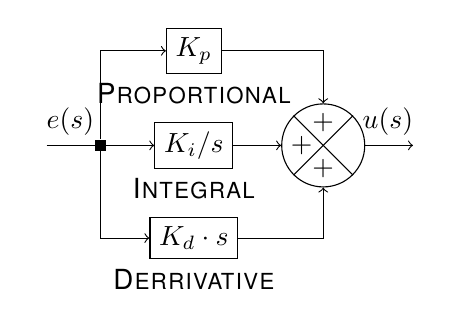
\begin{tikzpicture}[node distance=0.05\textwidth and 0.05\textwidth]
		\node (error) {};
		\node [fill,right=of error,rectangle,inner sep=2pt] (branch) {};
		\node [draw,right=of branch,rectangle] (i) {${K_i}/{s}$};
		\node [draw,above=of i,rectangle] (p) {$K_p$};
		\node [draw,below=of i,rectangle] (d) {${K_d}\cdot{s}$};
		\node [draw,right=of i,circle,minimum size=3em] (sum) {};
			\draw (sum.north west) -- (sum.south east);
			\draw (sum.north east) -- (sum.south west);
		\node [right=of sum] (output) {};

		\draw [->] (branch) |- (p);
		\draw [->] (error) -- (i);
		\draw [->] (branch) |- (d);
		\draw [->] (p) -| (sum);
		\draw [->] (i) -- (sum);
		\draw [->] (d) -| (sum);
		\draw [->] (sum) -- (output);

		\node [anchor=north] at (sum.north) {$+$};
		\node [anchor=west] at (sum.west) {$+$};
		\node [anchor=south] at (sum.south) {$+$};

		\node [anchor=south west] at (error) {$e(s)$};
		\node [anchor=south east] at (output) {$u(s)$};

		\node [anchor=north] at (p.south) {\textsc{Proportional}};
		\node [anchor=north] at (i.south) {\textsc{Integral}};
		\node [anchor=north] at (d.south) {\textsc{Derrivative}};
	\end{tikzpicture}
	\caption{Block diagram of a PID controller}
	\label{fig:pid}
\end{figure}

\section{Specification}

The transfer function for the industrial plant process $G(s)$ was given as follows:
\begin{equation} \label{eq:G}
	G(s) = \frac{s + 1}{s(s^2 + 4s + 5)}
\end{equation}
The transfer function $G_c(s)$ for the two controllers was chosen to meet the system performance specification detailed in Table~\ref{tab:spec}.

\begin{table}[h]
	\centering
	\footnotesize
	\begin{threeparttable}
		\caption{System perfomance specification.}
		\label{tab:spec}
		\begin{tabular}{@{}crrrr@{}}
			\toprule
			\textsc{Controller} &
				$M_0$[\%] &
				$T_r$[\si{\second}] &
				$T_{2\%}$[\si{\second}] &
				$SSE$[\%] \\
			\cmidrule(r){1-1}\cmidrule(l){2-5}
			1 &  5 & 1.0 &   4 & --- \\
			2 & 20 & 0.5 & --- &   5 \\
			\bottomrule
		\end{tabular}
	\end{threeparttable}
\end{table}

\section{Design}

\begin{figure}
	\centering
	\footnotesize
	\begin{tikzpicture}
		\begin{axis}[
			axis lines=center,
			xmin=-2.1,xmax=0.5,
			ymin=-5,ymax=5,
			xlabel={$\Re(s)$},ylabel={$\Im(s)$},
		]
			\addplot [thick,cyan]
				table [x={re1}, y={im1}] {data/rlocus.dat}
				node [draw,black,cross out,inner sep=1.7pt]
					at (current plot begin) {}
				node [draw,black,circle,inner sep=1.7pt]
					at (current plot end) {};
			\addplot [thick,cyan]
				table [x={re2}, y={im2}] {data/rlocus.dat}
				node [draw,black,cross out,inner sep=1.7pt]
					at (current plot begin) {}
				node [draw,black,circle,inner sep=1.7pt]
					at (current plot end) {};
			\addplot [thick,cyan]
				table [x={re3}, y={im3}] {data/rlocus.dat}
				node [draw,black,cross out,inner sep=1.7pt]
					at (current plot begin) {}
				node [draw,black,circle,inner sep=1.7pt]
					at (current plot end) {};
		\end{axis}
	\end{tikzpicture}
	\caption{Root locus of system poles from closed loop poles to closed loop zeros as $G_c$ varies from zero to infinity.}
	\label{fig:rlocus}
\end{figure}


\begin{figure}
	\centering
	\footnotesize
	\begin{tikzpicture}
		\begin{axis}[
			axis lines=center,
			xmin=-2.1,xmax=0.5,
			ymin=-5,ymax=5,
			xlabel={$\Re(s)$},ylabel={$\Im(s)$},
		]
			\addplot [thick,cyan]
				table [x={re1}, y={im1}] {data/rlocus.dat}
				node [draw,black,cross out,inner sep=1.8pt]
					at (current plot begin) {}
				node [draw,black,circle,inner sep=1.7pt]
					at (current plot end) {};
			\addplot [thick,cyan]
				table [x={re2}, y={im2}] {data/rlocus.dat}
				node [draw,black,cross out,inner sep=1.7pt]
					at (current plot begin) {}
				node [draw,black,circle,inner sep=1.7pt]	
					at (current plot end) {};
			\addplot [thick,cyan]
				table [x={re3}, y={im3}] {data/rlocus.dat}
				node [draw,black,cross out,inner sep=1.7pt]
					at (current plot begin) {}
				node [draw,black,circle,inner sep=1.7pt]
					at (current plot end) {};

			\addplot [ultra thick,red,restrict x to domain=-0.80058:-0.7103] 
				table [x={re1}, y={im1}] {data/rlocus.dat};
			\addplot [ultra thick,red,restrict x to domain=-1.6449:-1.5997]
				table [x={re2}, y={im2}] {data/rlocus.dat};
			\addplot [ultra thick,red,restrict x to domain=-1.6449:-1.5997]
				table [x={re3}, y={im3}] {data/rlocus.dat};
			\node [draw,thick,red!50!black,rectangle,inner sep=2pt]
				at (-0.75901,0) {};
			\node [draw,thick,red!50!black,rectangle,inner sep=2pt]
				at (-1.6205,-2.8132) {};
			\node [draw,thick,red!50!black,rectangle,inner sep=2pt]
				at (-1.6205,2.8132) {};

			\addplot [ultra thick,blue,restrict x to domain=-0.88392:-0.8242]
				table [x={re1}, y={im1}] {data/rlocus.dat};
			\addplot [ultra thick,blue,restrict x to domain=-1.5879:-1.558]
				table [x={re2}, y={im2}] {data/rlocus.dat};
			\addplot [ultra thick,blue,restrict x to domain=-1.5879:-1.558]
				table [x={re3}, y={im3}] {data/rlocus.dat};
			\node [draw,thick,blue!50!black,rectangle,inner sep=2pt]
				at (-0.85877,0) {};
			\node [draw,thick,blue!50!black,rectangle,inner sep=2pt]
				at (-1.5706,-3.7196) {};
			\node [draw,thick,blue!50!black,rectangle,inner sep=2pt]
				at (-1.5706,3.7196) {};
		\end{axis}
	\end{tikzpicture}
	\caption{Chosen closed loop, pole locations and acceptable margins for gain \textcolor{red!}{\textsc{controller} 1} and \textcolor{blue!}{\textsc{controller} 2}, marked on the root locus. Gain compensation only.}
	\label{fig:rlocus_Gc}
\end{figure}

\printbibliography

\end{document}
